%%%%%%%%%%%%%%%%%%%%%%%%%%%%%%%%%%%%%%%%%%%%%%%%%%%%%%%%%%%%%%%%%%%%%%%%%%%%%%%%%%%%%%%%%%%%%%%%%%%
%%%%%%%%%%%%%%%%%%%%%%%%%%%%%%%%%%%%%%%%%%%%%%%%%%%%%%%%%%%%%%%%%%%%%%%%%%%%%%%%%%%%%%%%%%%%%%%%%%%

\chapter*{Introducción}
\addcontentsline{toc}{chapter}{Introducción}

Gracias a los avances médicos del último siglo se ha incrementado la esperanza de vida y la calidad de vida. 
%
Desafortunadamente, también ha aumentado la presencia de enfermedades no-transmisibles asociadas con la edad. 
%
En México el sector de la población con más de 60 años de edad, considerados en alto riesgo para este tipo de enfermedades, contempló a 10 millones de personas en 2010, y en 2015 dicha cifra creció a 12 millones \cite{Censo10,Intercensal15}.

En este trabajo se destaca la demencia de entre las enfermedades asociadas con la edad.
%
La demencia consiste en el desarrollo de déficits cognoscitivos suficientemente graves como para interferir en las actividades laborales y sociales.
%
La demencia se considera irreversible y no se han identificado curas definitivas \cite{PlanAlzheimer04}, debido a lo cual ha surgido un gran interés en definir y diagnosticar sus etapas tempranas \cite{Knopman01}.
%
El deterioro cognitivo leve (PCL), considerado una etapa temprana de la demencia, se define como \textit{``una alteración adquirida y prolongada de una o varias funciones cognitivas, que no corresponde a un síndrome focal y que no cumple con criterios suficientes de gravedad para ser calificada como demencia"} \cite{Robles02}.
%
Por síndrome focal se entiende un daño en una estructura nerviosa específica y de causa conocida (como una hemorragia o una embolia) cuyo inicio sea inmediato y evidente; en cambio, el inicio del DCL es insidioso \cite{Petersen01}.

El DCL puede detectarse por medio de diversos métodos que pueden ser complementarios. 
%
La forma más sencilla de detectarlo es por la autopercepción de fallas en la memoria o por la percepción de otros;
es común que estos criterios subjetivos lleven a falsos negativos o falsos positivos, ésto por la percepción personal del nivel \textit{normal} de deterioro que se debe al envejecimiento.
%
Otras posibilidades para la detección incluyen la entrevista clínica de un especialista, o la aplicación de cuestionarios sobre dificultades en la memoria. 
%
Métodos más objetivos aún corresponden al diagnóstico con pruebas neuropsicológicas. 
%
Los análisis genéticos, químicos, de imágenes cerebral, entre otros, estudian el sistema nervioso central per se; dichas técnicas y otras, en combinación con las pruebas neuropsicológicas, permitirán diagnosticar más acertadamente el DCL y desentrañar los fenómenos neurobiológicos subyacentes.
%Técnicas genéticas, químicas o de imágenes cerebrales u otras en elaboración, que pueden ser o no muy costosas, en su combinación con las neuropsicológicas, permitirían diagnosticar más acertadamente el DCL así como desentrañar sus correlatos neurobiológicos. 

En este sentido, en el presente trabajo se busca desarrollar métodos para determinar el DCL con base en mediciones de la actividad eléctrica cerebral, muscular y ocular; se mantiene presente que el fenómeno del deterioro cognitivo (más allá del DCL) no puede reducirse exclusivamente a tales mediciones. 
%
Las conclusiones sobre las señales electrofisiológicas deben ser contrastadas siempre con los resultados de evaluaciones neuropsicológicas y revisiones neurológicas.

En concreto se utilizarán registros de varias señales electrofisiológicas --electroencefalograma (EEG), electrooculograma (EOG) y electromiograma (EMG)--, técnica conocida como polisomnografía (PSG)\footnote{La 
PSG puede contener otro tipo de señales como electrocardiograma, niveles de oxígeno en la sangre, 
esfuerzo respiratorio, movimiento de las piernas, entre otras}, obtenidas durante 
etapas específicas en el sueño del paciente.
%%ANADÏ ESTO, checar para qué figura queda, porque debe especificarse que comunmente en la PSG se registran 2 electrodos, C3 y C4, emg y ojos. Sin embargo, como el objetivo es conocer la actividad eléctrica cerebral de más regiones, se colocaron 19 electrodos en la cabeza de cada paciente, dispuestos según el sistema 10/20. ESTO DEBE ESTAR EN EL PIE DE FIGURA CORRESPONDIENTE. NO ME ACUERDO SI ESTÁ O NO, PERO FUE QUE NOS PIDIERON QUE EXPLICARAS MÁS...Y LO DE LAS OREJAS CORTOCIRCUITADAS. CITA AL MANUAL DE NIEDERMEYER
%
Conviene destacar que muchos de los marcadores para el DCL definidos con base en el EEG dependen
efectivamente de su respectivo espectro de potencia%%ANADÏ ESTO: y que normalmente estos marcadores electrofisiológicos se obtienen durante un estado de vigilia en reposo, es decir, despierto con ojos cerrados AGREGAR AQUÍ VARIAS REFS QUE ESTÁN AQUÍ ABAJITO  \cite{ Prichep et al., 1994; Rossini et al., 2006; Prichep et al., 2006; Rossini et al., 2008}. En general, se encontró que la potencia absoluta (PA) y relativa (PR) es mayor en la frecuencia de theta en estos pacientes y hay una correlación positiva con delta a más deterioro cognitivo en amplias regiones cerebrales y además la estabilidad de las fuentes de alfa en regiones posteriores sirve como un predictor confiable (Babiloni et al., 2013). Estos patrones se cree que representan alteraciones en el hipocampo relacionadas al deterioro cognitivo. 
EEG está asociado al grado de actividad cerebral en términos de energía, entonces el espectro de 
potencias explica \textit{cómo} es dicha actividad.%, pero esta última frase se puede quitar.
%Montplaisir   citar aquí de la tesis de Gén la referencia, Julito, x fa hallan que el sueño MOR es mejor predictor que la vigilia
%Babiloni C, Carducci F, Lizio R, Vecchio F, Baglieri A, Bernardini S, Cavedo S,  Bozzao A, Buttinelli C, Esposito F, Giubilei F, Guizzaro A, Marino S , Montella P, Quattrocchi QC, Redolfi A, Soricelli A, Tedeschi G, Ferri R, Rossi-Fedele G, Ursini F, Scrascia F, Vernieri F, Pedersen TJ, Hardemark HG, Rossini PM, Frisoni GB (2013). Resting state cortical electroencephalographic rhythms are related to gray matter volume in subjects with mild cognitive impairment and Alzheimer´s disease. Human brain mapping, 34, 1427-1446.
%Prichep LS, John ER, Ferris SH, Rausch L, Fang Z, Cancro R, Torossian C, Reisberg B (2006). Prediction of longitudinal cognitive decline in normaly elderly with subjective complaints using electrophysiological imaging. Neurobiology and aging, 27, 471-481.
%Prichep LS, John ER, Ferris SH, Reisberg B, Almas M, Alper K, Cancro R (1994). Quantitative EEG correlates of cognitive deterioration in the elderly. Neurobiology and aging, 15, 85-90.

El presente trabajo toma parte en el problema metodológico de que las señales electrofisiológicas típicamente representan procesos no--lineales y no--estacionarios, y sin 
embargo suelen ser analizadas usando herramientas que suponen linealidad y estacionariedad. Se sabe que
las señales biológicas son mayormente no estacionarias, pero en ventanas pequeñas de tiempo éstas son
mayormente estacionarias.%AQUÍ PUEDEN PONER LA FIGURA DEL ARTÍCULO.
Además estudios previos han demostrado que señales mayores de 20 segundos pueden ayudar 
a inferir problemas neurológicos \cite{Cohen77}.
%
En el caso particular del espectro de potencias, es común que sea calculado usando la 
transformada de Fourier sobre segmentos cortos para evitar los \textit{efectos} de la 
no--estacionariedad \cite{Kaiser00}.
%
Es por ello que se buscan herramientas para verificar la estacionariedad débil (más detalles en 
la sección de métodos)  en los registros electrofisiológicas, y con especial atención en la 
posibilidad de que puedan usarse como marcadores de deterioro cognitivo.
%No se conocen otros estudios que empleen la prueba de Priestley-Subba-Rao (ref) que se explicará más adelante para probar estacionariedad con excepción de Rosales-Lagarde et al. (2017), sin embargo aquí se muestra con una mayor precisión.
%Rosales-Lagarde, A., Rodríguez-Torres, E.E., Enciso-Alva, J., Martínez-Alcalá, C., Vázquez-Tagle, G., Tetlamatzi-Montiel, M., Viveros, J. and López-Noguerola, J.S. (2017). Stationarity during REM sleep in Old Adults. Alzheimer´s and Dementia, P723-P724. doi: http://dx.doi.org/10.1016/j.jalz.2017.06.937

En este trabajo se definirá al Posible Deterioro Cognitivo Leve (PDCL) como una disminución de las funciones cognitivas del sujeto con respecto las típicas de su edad y nivel de educación. 
%
El desempeño de las funciones cognoscitivas es medido de acuerdo a la prueba neuropsicológica Neuropsi [citar? ostrosky]. 
%
Se entiende el déficit en estas funciones como mediciones por debajo de la media menos 3 desviaciones estándar de las mediciones típicas para el grupo de edad y nivel de educación, según la validación de la prueba para México [citar].
%arreglar la cita. Es decir, se espera hallar marcadores en la actividad eléctrica cerebral, muscular u ocular correlacionados con los déficits en alguna o varias funciones neuropsicológicas. Se usa el término de probable para ser congruentes con las especificaciones sobre los métodos, es decir, porque los análisis que se presentan pretenden arrojar mayores indicios anatómicos y fisiológicos sobre lo ya detectado con las pruebas.
%Ostrosky-Solís, F. Ardila, A. & Rosselli, M. (1999). Neuropsi: A brief neuropsychological test battery in Spanish with norms by age and educational level. Journal of the International Neuropsychological Society, 5, 413-433.

%%%%%%%%%%%%%%%%%%%%%%%%%%%%%%%%%%%%%%%%%%%%%%%%%%%%%%%%%%%%%%%%%%%%%%%%%%%%%%%%%%%%%%%%%%%%%%%%%%%
%%%%%%%%%%%%%%%%%%%%%%%%%%%%%%%%%%%%%%%%%%%%%%%%%%%%%%%%%%%%%%%%%%%%%%%%%%%%%%%%%%%%%%%%%%%%%%%%%%%

\section*{Antecedentes}
\addcontentsline{toc}{section}{Antecedentes}

El sueño MOR ha sido ampliamente relacionado con la consolidación de la memoria, así como con
otras funciones cognitivas como la integración de conocimientos aprendidos durante la vigilia y las funciones ejecutivas
\cite{Fishbein1971,Fishbein1977,Lucero1970,Pearlman1971,Pearlman1974,Smith1991}.%Añadir a Corsi-Cabrera et al. (2015).
%Corsi-Cabrera, M., Rosales-Lagarde, A., Del Río-Portilla, Y., Sifuentes-Ortega, R., Alcántara-Quintero, B. (2015). Effects of selective REM sleep deprivation on prefrontal gamma activity and executive functions. International journal of psychophysiology, 96, 115-124, doi: 10.1016/j.ijpsycho.2015.02.027. 
En el caso de adultos mayores, la correlación entre deterioro cognitivo y trastornos del sueño ha 
sido reportada por varios autores a partir de estudios poblacionales 
\cite{Amer13,Miyata13,Reid06,Potvin12}.
%
Tal correlación era de esperarse ya que los procesos de atención y memoria, por ejemplo, dependen de 
los circuitos colinérgicos activados durante el sueño MOR \cite{Braun1997}; y estos circuitos son 
propensos a degradación estructural tanto en el envejecimiento normal como en el patológico,  y 
especialmente en el segundo \cite{Schliebs11}.

En 2016 Vázquez-Tagle y colaboradores estudiaron el PDCL en adultos mayores del estado de Hidalgo con el método no lineal del Análisis de Fluctuaciones sin Tendencia (DFA, por sus siglas en inglés), encontrando efectivamente que los sujetos con PDCL presentan mayor ruido browniano en varias regiones en comparación con los pacientes sin PDCL\cite{VazquezTagle16}.
%
Adicionalmente, la sugerencia de que sujetos con alteraciones neurológicas y deterioro cognitivo exhiben estacionariedad débil en sus 
registros de EEG en mayor proporción (respecto a individuos sanos) fue sugerida anteriormente
\cite{Cohen77}; aquél análisis se 
refiere a su vez a trabajos anteriores sobre estacionariedad y normalidad en registros de EEG
\cite{McEwen75,Sugimoto78,Kawabata73}.
%
Los estudios referidos se enmarcan en un primer intento de verificar que los registros 
electrofisiológicos no pueden modelarse como señales \textit{simples} (lo contrario a señales 
complejas).
%
%El tema de la estacionariedad en señales parece relevante nuevamente a la luz de una revisión
%por Kreuz y colaboradores \cite{Kreuz07}, según la cual el método más eficaz para detectar 
%correlación es la correlación \textit{clásica} --en comparación con algunos métodos basados en 
%entropía o información mutua, por ejemplo. 
%%
%Para llegar a tal conclusión analizaron algunos tipos \textit{comunes} de datos, experimentales y 
%simulados, así como algunos tipos comunes de perturbaciones. Un resultado tan controversial provoca replantearse, por ejemplo, si algún método en particular es 
%adecuado para un tipo arbitrario de datos, o si algunas generalizaciones para estos métodos son 
%efectivamente necesarias.

El presente trabajo tiene el objetivo de identificar concretamente
los posibles cambios en los registros de PSG  debidos al PDCL. Siguiendo a Cohen \cite{Cohen77}, es posible predecir que en sujetos con PDCL habrá menores porcentajes de épocas estacionarias en comparación con sujetos controles, lo que puede deberse a una mayor cantidad de ondas lentas. Sin embargo, en esta tesis sólo se explorará si la primera condición se cumple, verificando el comportamiento estacionario de los registros.%CHECAR SI ASÍ ESTÁ BIEN DICHO...

%%%%%%%%%%%%%%%%%%%%%%%%%%%%%%%%%%%%%%%%%%%%%%%%%%%%%%%%%%%%%%%%%%%%%%%%%%%%%%%%%%%%%%%%%%%%%%%%%%%
%%%%%%%%%%%%%%%%%%%%%%%%%%%%%%%%%%%%%%%%%%%%%%%%%%%%%%%%%%%%%%%%%%%%%%%%%%%%%%%%%%%%%%%%%%%%%%%%%%%

En un estudio reciente, EEG de una noche polisomnografía de personas mayores con y sin deterioro cognitivo según las evaluaciones con el Neuropsi analizó el porcentaje de estacionariedad.  En sueño MOR el porcentaje fue menor que el del sueño NMOR y la vigilia, se obtuvo estacionariedad  como un índice para comparar NMOR versus sueño MOR en ambos grupos \cite{ROSALESLAGARDE2017}.

%El sueño MOR ha sido ampliamente reconocido como parte de la consolidación de la memoria, así como
%otras funciones cognitivas 
%\cite{Fishbein1971,Fishbein1977,Lucero1970,Pearlman1971,Pearlman1974,Smith1991}.
%%
%En el caso de adultos mayores, la correlación entre deterioro cognitivo y trastornos del sueño ha 
%sido reportada por varios autores a partir de estudios poblacionales 
%\cite{Amer13,Miyata13,Reid06,Potvin12}.
%%
%Tal correlación era de esperarse ya que los procesos de atención y memoria, por ejemplo, dependen de 
%los circuitos colinérgicos activados durante el sueño MOR \cite{Braun1997}; estos circuitos son 
%propensos a degradación estructural tanto en el envejecimiento normal como en el patológico,  y 
%especialmente en el segundo \cite{Schliebs11}.
%
%En 2016 Vázquez-Tagle y colaboradores estudiaron la epidemiología del DCL en adultos mayores dentro 
%del estado de Hidalgo y su posible relación con trastornos de sueño, encontrando efectivamente una 
%correlación entre una menor eficiencia del sueño (porcentaje de tiempo de sueño respecto al tiempo 
%en cama) y la presencia de deterioro cognitivo \cite{VazquezTagle16}.
%%
%En aquél estudio se efectuaron registros de PSG para algunos de los participantes, con la intención 
%de verificar que existen diferencias en los registros correspondientes a individuos con y sin DCL.
%%
%El presente trabajo se enmarca dentro de una reciente colaboración, con el objetivo de identificar concretamente
%los posibles cambios en los registros de PSG  ocurridos durante el DCL o PDC.
%
%La idea de que sujetos con deterioro cognitivo exhiban cambios en sus registros de PSG relacionados 
%a la estacionariedad débil, fue sugerida por Cohen en 1977 \cite{Cohen77}; aquél análisis se 
%refiere a su vez a trabajos anteriores sobre estacionariedad y normalidad en registros de EEG
%\cite{McEwen75,Sugimoto78,Kawabata73}.
%%
%Los estudios referidos se enmarcan en un primer intento de verificar que los registros 
%electrofisiológicos no pueden modelarse como señales \textit{simples} (lo contrario a señales 
%complejas).
%%
%%El tema de la estacionariedad en señales parece relevante nuevamente a la luz de una revisión
%%por Kreuz y colaboradores \cite{Kreuz07}, según la cual el método más eficaz para detectar 
%%correlación es la correlación \textit{clásica} --en comparación con algunos métodos basados en 
%%entropía o información mutua, por ejemplo. 
%%%
%%Para llegar a tal conclusión analizaron algunos tipos \textit{comunes} de datos, experimentales y 
%%simulados, así como algunos tipos comunes de perturbaciones.
%%
%%Un resultado tan controversial provoca replantearse, por ejemplo, si algún método en particular es 
%%adecuado para un tipo arbitrario de datos, o si algunas generalizaciones para estos métodos son 
%%efectivamente necesarias.

%%%%%%%%%%%%%%%%%%%%%%%%%%%%%%%%%%%%%%%%%%%%%%%%%%%%%%%%%%%%%%%%%%%%%%%%%%%%%%%%%%%%%%%%%%%%%%%%%%%
%%%%%%%%%%%%%%%%%%%%%%%%%%%%%%%%%%%%%%%%%%%%%%%%%%%%%%%%%%%%%%%%%%%%%%%%%%%%%%%%%%%%%%%%%%%%%%%%%%%

\section*{Pregunta de investigación y objetivos}
\addcontentsline{toc}{section}{Pregunta de investigación y objetivos}

¿Las series de tiempo de los registros de polisomnografía en adultos mayores son débilmente estacionarias?
%
Si en efecto, son débilmente estacionarias ¿Ésta es distinta entre los sujetos con PDCL y sin PDCL?

%%%%%%%%%%%%%%%%%%%%%%%%%%%%%%%%%%%%%%%%%%%%%%%%%%%%%%%%%%%%%%%%%%%%%%%%%%%%%%%%%%%%%%%%%%%%%%%%%%%
%%%%%%%%%%%%%%%%%%%%%%%%%%%%%%%%%%%%%%%%%%%%%%%%%%%%%%%%%%%%%%%%%%%%%%%%%%%%%%%%%%%%%%%%%%%%%%%%%%%

\subsection*{Hipótesis}

Existen diferencias en la estacionariedad débil de la actividad eléctrica cerebral, muscular u ocular en adultos mayores con PDCL respecto a 
individuos sanos. 
\textit{presencia} deen registros de PSG.

%%%%%%%%%%%%%%%%%%%%%%%%%%%%%%%%%%%%%%%%%%%%%%%%%%%%%%%%%%%%%%%%%%%%%%%%%%%%%%%%%%%%%%%%%%%%%%%%%%%

\subsection*{Objetivo general}

Buscar pruebas estadísticas formales para detectar si una serie de tiempo dada procede de un 
proceso estocástico débilmente estacionario.
%
Usar tales pruebas sobre registros de PSG en adultos mayores para investigar si la 
presencia de más segmentos débilmente estacionarios se asocia con la condición de PDCL.

%%%%%%%%%%%%%%%%%%%%%%%%%%%%%%%%%%%%%%%%%%%%%%%%%%%%%%%%%%%%%%%%%%%%%%%%%%%%%%%%%%%%%%%%%%%%%%%%%%%

\subsection*{Objetivos específicos}

\begin{itemize}
\item Estudiar la definición de estacionariedad para procesos estocásticos.

\item Investigar cómo detectar, como prueba de hipótesis, si una serie de tiempo dada proviene
de un proceso estocástico débilmente estacionario, y bajo qué supuestos 
es válida dicha caracterización.

\item Establecer si los registros de PSG durante las etapas de sueño son débilmente estacionarios.

\item Investigar si la presencia de segmentos estacionarios en los registros es diferente si la
PSG corresponde a un individuo con PDCL.
\end{itemize}


\section*{Sobre la estructura del texto}
\addcontentsline{toc}{section}{Sobre la estructura del texto}

%Debido a la naturaleza multidisciplinaria del presente trabajo, se ha estructurado de manera que %resalten los temas teóricos más como objetos abstractos que como componentes de herramientas para el análisis de datos.

El presente trabajo está conformado por 6 capítulos y un apéndice. El primer capítulo aborda conceptos preliminares como medida, integración, variables aleatorias, estimadores, pruebas de hipótesis, proceso estocásticos, espacios de Hilbert y la transformada de Fourier.

%El objeto principal de este trabajo es el estudio de la estacionariedad débil en registros de polisomnograma de adultos mayores para investigar si es posible usarlos para

En el segundo capítulo se expone una serie de temas relacionados con la \textit{estadística en el dominio espectral}, es decir, obtener el espectro de potencias de un proceso estocástico --particularmente de procesos débilmente estacionarios.
%
Debido a la notoria relación mutua entre estos temas, se decidió ilustrar en la figura \ref{intro:estructura} la red de temas según dependen unos de otros.

En el tercer capítulo se expone el \textit{espectro evolutivo}, una generalización del espectro de potencias para procesos no estacionarios.
%
Como el espectro evolutivo de un proceso débilmente estacionario se reduce al espectro de potencias, se describe una metodología para detectar estacionariedad débil.

%
%Naturalmente, esta tarea implica la exposición de varios otros temas relativos a las condiciones bajo las cuales el espectro de potencias está bien definido, así como las condiciones bajo las cuales es posible su estimación.

%El objetivo final del capítulo es presentar una prueba de estacionariedad débil y que es usada para estudiar las propiedades de los registros.

En el cuarto capítulo se presentan conceptos preliminares de índole fisiológica como detección de deterioro cognitivo y su relación con el sueño. En particular se explora el estudio del sueño a través de la polisomnografía.

En el capítulo quinto describe cómo se aplica la metodología descrita en los capítulos anteriores.
%
Los registros son divididos en segmentos, llamados \textit{épocas}, que son analizadas en tres niveles:
\begin{itemize}
\item Se prueba la homogeneidad de cada época
\item Se estudian las características de las distintas épocas dentro 
\end{itemize}

En el capítulo sexto se discuten los resultados obtenidos y se exponen las conclusiones.

%En el capítulo 2 se describe lo  que es el deterioro cognitivo leve y cómo se detecta a nivel de comportamiento, así como se describen varios esfuerzos por detectar este padecimiento en base a mediciones más objetivas a nivel de sistema (en particular, con el enfoque de mediciones de la actividad cerebral). 
%
%Dado que se ha reportado relaciones entre el sueño MOR y la memoria a corto y largo plazo, se dedica una sección a describir el sueño y sus características, y su estudio a través de la polisomnografía.
%
%En el capítulo 3 se muestran los sujetos de estudio; debido a que el trabajo se enmarca en una colaboración, se describe la metodología usada en trabajos anteriores usando esta misma base datos, y se considera como conocidos los datos sobre pruebas neuropsicológicas y los registros de PSG se consideran conocidos. 
%%
%Posteriormente se expone la metodología original en este trabajo correspondiente en cuanto el uso que se da a la prueba de PSR. El análisis se efectúa en dos niveles: 
%\begin{itemize}
%\item Para cada sujeto, los registros son segmentados en una colección de ventanas (épocas) que se clasifican como etapas según sus características tipificadas\footnote{Estas características son en su mayoría visuales, y se encuentran reguladas por lineamientos internacionales como aquél de la AASM \cite{AASM07}} , debido a la heterogeneidad del sueño, tiene sentido tratar a estas épocas como una población
%\item A nivel de grupo, algunas características son comparadas entre sujetos
%\end{itemize}
%conviene destacar que la heterogeneidad en los registros puede observarse intuitivamente de manera gráfica.

\begin{figure}
\centering
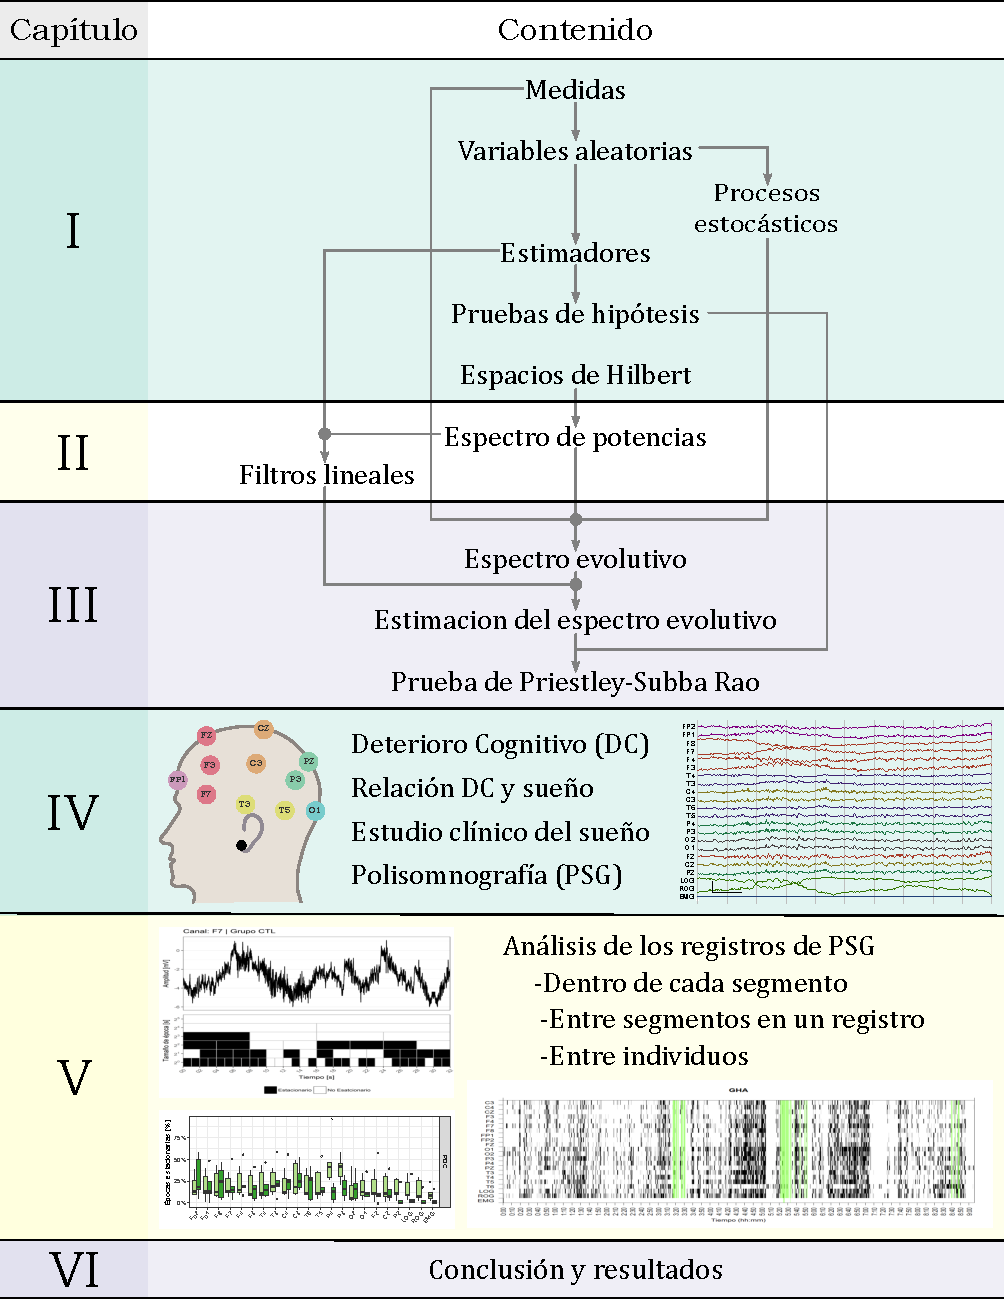
\includegraphics[width=.9\textwidth]{./estructura_texto_v2.pdf}
\caption[Estructura de la tesis]{Se ilustra gráficamente las \textit{dependencias} respecto a los tópicos de matemáticas, es decir, los temas que deben discutirse antes que otros. El resto del texto (incluyendo los tópicos de fisiología) son expuesto de forma más \textit{secuencial}, por lo que no se consideró necesario ilustrar sus dependencias.}
\label{intro:estructura}
\end{figure}

%%%%%%%%%%%%%%%%%%%%%%%%%%%%%%%%%%%%%%%%%%%%%%%%%%%%%%%%%%%%%%%%%%%%%%%%%%%%%%%%%%%%%%%%%%%%%%%%%%%
%%%%%%%%%%%%%%%%%%%%%%%%%%%%%%%%%%%%%%%%%%%%%%%%%%%%%%%%%%%%%%%%%%%%%%%%%%%%%%%%%%%%%%%%%%%%%%%%%%%